%----------------------------------------------------------------------------------------
%	METODE
%----------------------------------------------------------------------------------------
\section*{METODE PENELITIAN}

\subsection*{Data Penelitian}

Data yang digunakan pada penelitian ini adalah data ontologi gen yang berasal dari situs geneontology.org.

\subsection*{Tahapan Penelitian}

Tahapan-tahapan yang dilakukan pada penelitian ini mengacu pada metode pengembangan aplikasi SW-OODM. Tahapan pengembangan aplikasi SW-OODM dapat dilihat pada Gambar \ref{fig:tahapan_penelitian}.

\begin{figure}[h!] % Gunakan \begin{figure*} untuk memasukkan Gambar
	\centering
	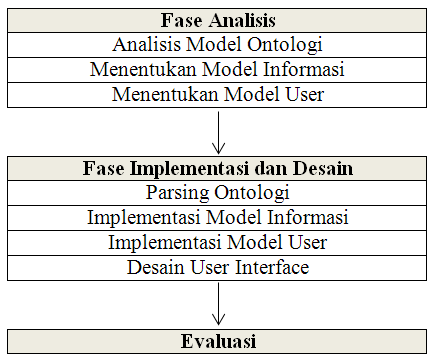
\includegraphics[width=200pt]{kolokium_tahapan_penelitian_gb2.png}
	\caption{Tahapan Penelitian}
	\label{fig:tahapan_penelitian}
\end{figure}

Fase Analisa

Pada fase analisa terdapat 3 aktivitas yang akan dilakukan, yaitu analisis model ontologi, menentukan model informasi, menentukan model user. Aktivitas analisis model ontologi akan diidentifikasi domain yang terdapat pada ontologi gen. Hasil identifikasi model ontologi digambarkan dengan bentuk graph, sehingga bentuk dari ontologi gen akan dapat lebih mudah dipelajari.

Aktivitas menentukan model informasi akan memanfaatkan hasil dari analisis model ontologi untuk menentukan kelas, atribut dan keterkaitan antar objek yang ada di dalam ontologi. Hal ini perlu dilakukan untuk menjadi acuan dalam pembuatan query dan membuat query yang tepat dengan SPARQL untuk mengambil informasi yang terdapat di dalam ontologi dan juga melakukan inferensi pengetahuan tumbuhan yang ada di dalam ontologi. 

Pada aktivitas menentukan model user akan dianalisis kebutuhan dari user yang akan menggunakan sistem yaitu berupa kelompok user yang mengakses sistem, rancangan kelas dari sistem, alur akivitas yang dilakukan user dan skenario alur akses sistem dari user. Hasil dari tahapan ini berupa definisi diagram use case, class diagram, activitiy diagram dan sequence diagram.

Fase Implementasi dan Desain

Pada fase implementasi dan desain akan diawali dengan parsing ontologi. Parsing ontologi memetakan ontologi gen menjadi triple yang berupa subject, predicate dan object. Setelah ontologi dilakukan parsing dan menghasilkan triple, hasil ini yang akan dilakukan query dengan menggunakan SPARQL.

Pada tahapan implementasi model informasi mencakup pembuatan query SPARQL untuk mengembalikan informasi yang terdapat dalam ontologi, yaitu informasi gene-product, cellular location dan sequence. Kemudian pada tahapan implementasi model akan dibuat fungsi-fungsi yang akan memanfaatkan query yang telah dibuat pada tahap implementasi model sehingga informasi dari sistem ontologi gen dapat diakses dengan menggunakan web. 

Pada tahapan implementasi user akan menghasilkan fungsi-fungsi yang akan menangani input yang diberikan oleh user, melakukan pengambilan informasi berdasarkan input yang diterima, dan memberikan output yang sesuai dengan input yang sudah diberikan. Tahap desain user interface akan menghasilkan halaman yang akan diakses oleh user. Halaman yang dibuat berupa halaman input dan halaman output yang dapat dilihat oleh user.

Evaluasi

Fase evaluasi akan dilakukan pengujian dari sistem yang sudah dibuat. Pengujian yang dilakukan  menggunakan metode black box. Metode ini akan memberikan kasus untuk dilakukan oleh sistem dengan memberi input dan menguji kesesuaian hasil yang diberikan oleh sistem.

\subsection*{Lingkungan Pengembangan}

Pembangunan sistem ontologi gen tanaman berbasis web ini dilakukan dengan menggunakan perangkat keras dan perangkat lunak sebagai berikut:

\begin{itemize}
	\item Prosesor Intel Core i7 4500U 1,8 GHz
	\item Memori 12 GB
	\item Hard disk 1 TB
	\item Sistem operasi Windows 7 Ultimate
	\item Bahasa pemrograman Python dengan Flask sebagai web framework
	\item RDFLib sebagai library yang digunakan untuk penggunaan RDF pada Phyton
	\item Lingkungan pengembangan (IDE) Visual Studio 2013 
	\item Protégé 4.3.0 sebagai pemodelan ontologi
\end{itemize}

\subsection*{Rencana Jadwal Penelitian}

Penelitian ini akan dilakukan selama 6 bulan dengan rincian kegiatan seperti tercantum pada Tabel \ref{tab:jadwal}.

\begin{table*}[h!]
	\begin{center}
		\caption{Rencana Jadwal Penelitian}
		\label{tab:jadwal}
		\footnotesize
		\begin{tabular}{|l|c|c|c|c|c|c|c|c|c|c|c|c|c|c|c|c|c|c|c|c|c|c|c|c|}
			\hline
			\multirow{2}{*}{Kegiatan}&\multicolumn{2}{c|}{Mei}&\multicolumn{4}{c|}{Juni}&\multicolumn{4}{c|}{Juli}&\multicolumn{4}{c|}{Agustus}&\multicolumn{4}{c|}{September}&\multicolumn{4}{c|}{Oktober}&\multicolumn{2}{c|}{November}\\
			\cline{2-25}
			&3&4&1&2&3&4&1&2&3&4&1&2&3&4&1&2&3&4&1&2&3&4&1&2\\
			\hline
			Penyusunan Proposal Skripsi&\cellcolor{black}&\cellcolor{black}&\cellcolor{black}&\cellcolor{black}&\cellcolor{black}&&&&&&&&&&&&&&&&&&&\\
			\hline
			Kolokium&&&&&&\cellcolor{black}&&&&&&&&&&&&&&&&&&\\
			\hline
			Pengumpulan Data&\cellcolor{black}&\cellcolor{black}&\cellcolor{black}&\cellcolor{black}&\cellcolor{black}&\cellcolor{black}&&&&&&&&&&&&&&&&&&\\
			\hline
			Fase Analisis&&&&&&&\cellcolor{black}&\cellcolor{black}&&&&&&&&&&&&&&&&\\
			\hline
			Fase Implementasi data&&&&&&&&&\cellcolor{black}&\cellcolor{black}&\cellcolor{black}&\cellcolor{black}&\cellcolor{black}&\cellcolor{black}&\cellcolor{black}&\cellcolor{black}&&&&&&&&\\
			\hline
			Fase Evaluasi&&&&&&&&&&&&&&&&&\cellcolor{black}&\cellcolor{black}&&&&&&\\
			\hline
			Penulisan Skripsi&&&&&&&&&\cellcolor{black}&\cellcolor{black}&\cellcolor{black}&\cellcolor{black}&\cellcolor{black}&\cellcolor{black}&\cellcolor{black}&\cellcolor{black}&\cellcolor{black}&\cellcolor{black}&\cellcolor{black}&&&&&\\
			\hline
			Seminar&&&&&&&&&&&&&&&&&&&&\cellcolor{black}&&&&\\
			\hline
			Sidang skripsi&&&&&&&&&&&&&&&&&&&&&&\cellcolor{black}&&\\
			\hline
			Perbaikan laporan penelitian&&&&&&&&&&&&&&&&&&&&&&&\cellcolor{black}&\cellcolor{black}\\
			\hline
		\end{tabular}
		\normalsize
	\end{center}
\end{table*}